\documentclass{scrreprt}
\setcounter{secnumdepth}{5}
\usepackage{listings}
\usepackage{enumitem}
\usepackage{underscore}
\usepackage{graphicx}
\usepackage[bookmarks=true]{hyperref}
\usepackage[utf8]{inputenc}
\usepackage[english]{babel}
\usepackage[pass,letterpaper]{geometry}
\usepackage[export]{adjustbox}
\usepackage{subcaption}
\usepackage{float}
\usepackage{longtable}

\graphicspath{{/home/mitansh/assemblerDoc/images/}}
\hypersetup{
    bookmarks=false,    % show bookmarks bar?
    pdftitle={Assembler Linker Loader Documentation},    % title
    pdfauthor={Akul Agrawal, Sujoy Ghosh, Mitansh Jain},                     % author
    pdfsubject={TeX and LaTeX},                        % subject of the document
    pdfkeywords={TeX, LaTeX, graphics, images}, % list of keywords
    colorlinks=true,       % false: boxed links; true: colored links
    linkcolor=black,       % color of internal links
    citecolor=black,       % color of links to bibliography
    filecolor=black,        % color of file links
    urlcolor=purple,        % color of external links
    linktoc=all            % only page is linked
}                                          %
\def\myversion{1.0}
\date{}
\title{}
\begin{document}
\begin{flushright}
    \rule{16cm}{5pt}\vskip1cm
    \begin{bfseries}
        \Huge{CS-244\\Assembler Linker Loader Documentation}\\
        \vspace{1.5cm}
        for\\
       
        \vspace{1.5cm}
        
         System Programming\\
        Lab\\
        \vspace{1.9cm}
        \LARGE{Prepared by: }\\
        Group-12\\
        Mitansh Jain - 160101042\\
        Sujoy Ghosh - 160101073\\
        Akul Agrawal - 160101085\\
        \vspace{1.9cm}
    \end{bfseries}
\end{flushright}
\tableofcontents
\listoffigures
\listoftables

\chapter{Introduction}
This is a documnatation made for how to use the assembler, linker, loader web based simulartor and about its working.\\
Documentation consists mainly of following segemnts:
\begin{enumerate}
\item Firstly document covers on how to use the simulator and how it works.
\item Then it covers working of following:
\begin{itemize}
\item[•] Assembler
\item[•] Linker
\item[•] Loader
\end{itemize}
\item Also it covers various features of the c-type language implemented.
\end{enumerate}

\chapter{Simulator}
\section{File Upload}
\begin{figure}[H]
\centering
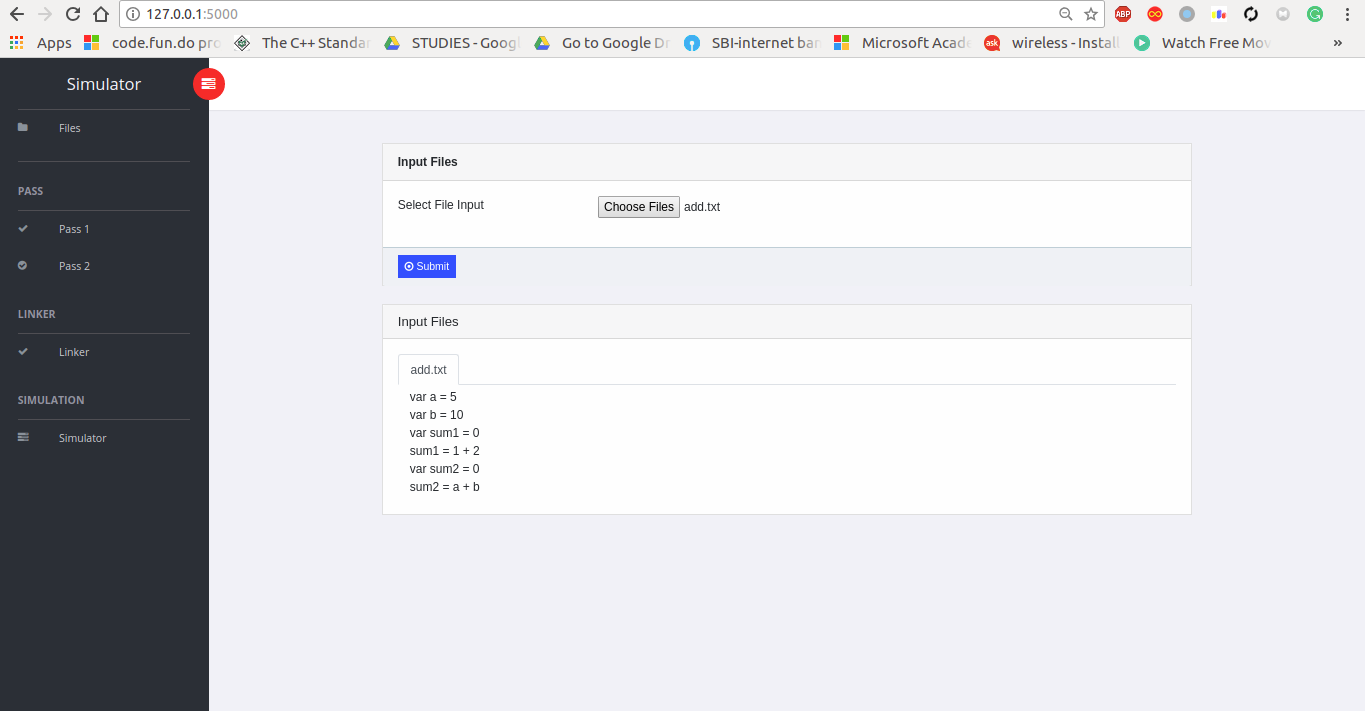
\includegraphics[width=\textwidth, keepaspectratio]{fileUpload.png}
\caption{File upload window}
\end{figure}
This is the first screen of our webbased simuator, it is used to upload file to be simulated. To use it:
\begin{itemize}
\item[•] Click on "Choose Files" button
\item[•] Then click submit button to upload files.
\item[•] After clicking on submit button contents of selected files will be visible below it.
\end{itemize}

After this to see output of assembler's pass1, pass2 or linker click on repective button on side nav bar.
After clicking on them following screens show up.

\section{Pass1 and Pass2}
\begin{figure}[H]
\centering
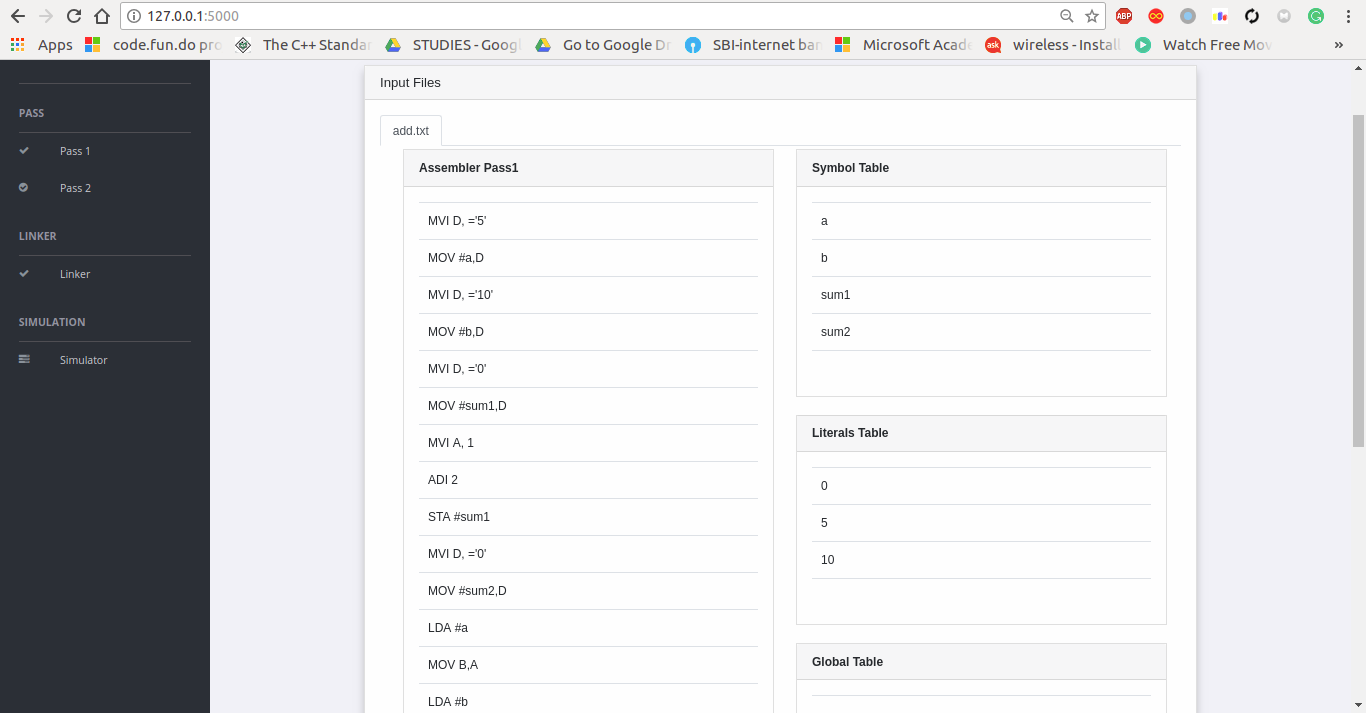
\includegraphics[width=\textwidth, keepaspectratio]{pass1.png}
\caption{Pass1 assembly, symbol table, literal table and global table}
\end{figure}

\begin{figure}[H]
\centering
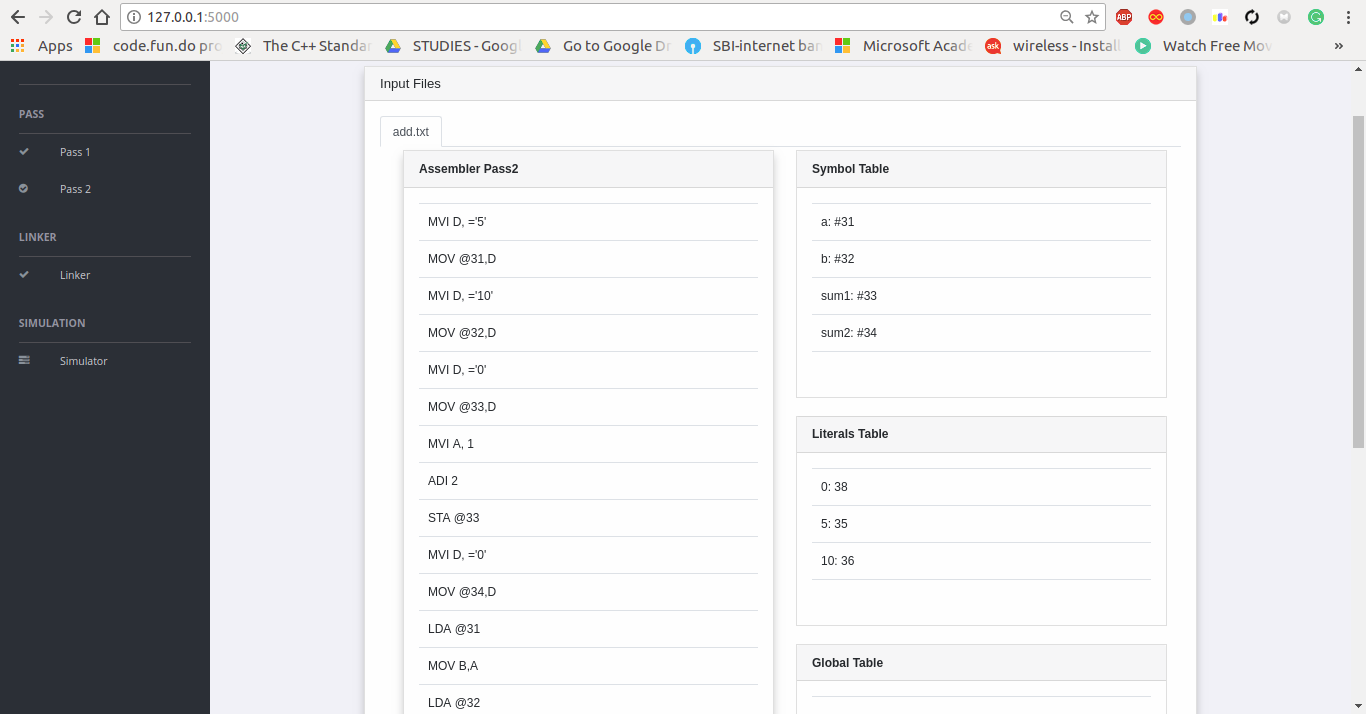
\includegraphics[width=\textwidth, keepaspectratio]{pass2.png}
\caption{Pass2 assembly, symbol table, literal table and global table}
\end{figure}

\section{Linker}
\begin{figure}[H]
\centering
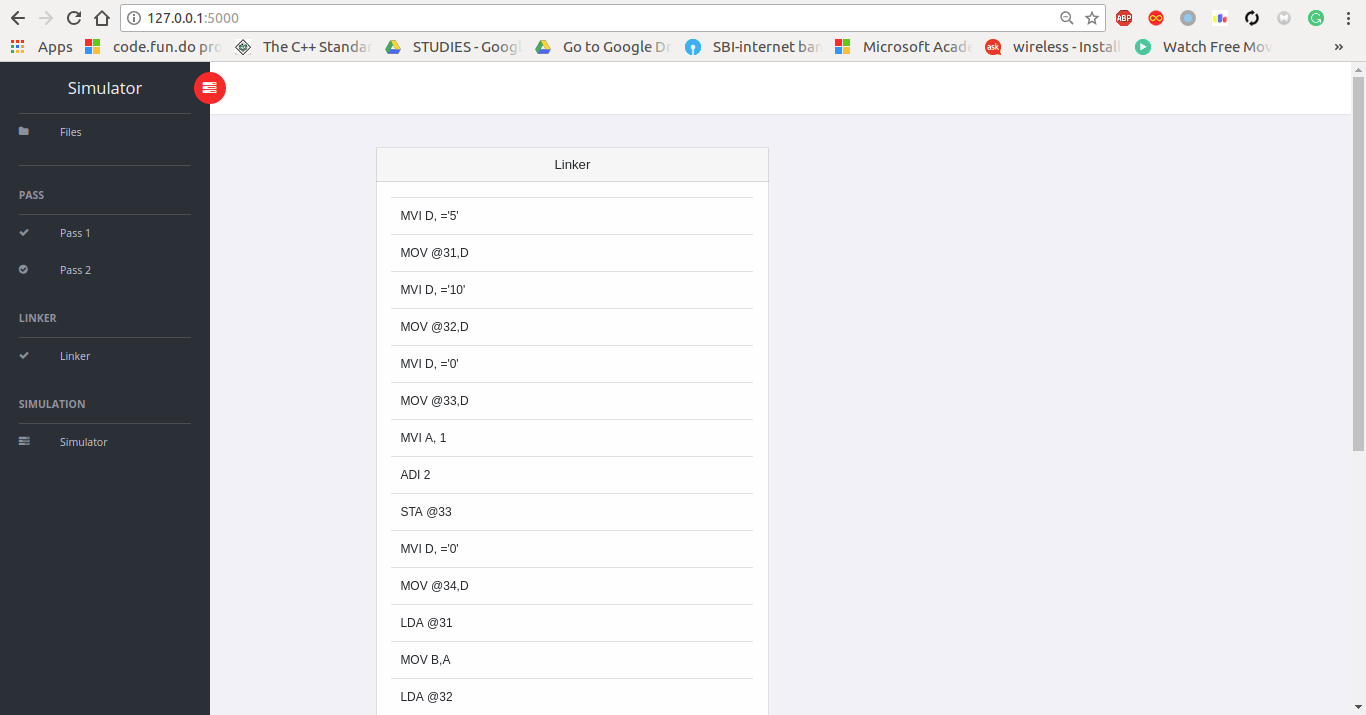
\includegraphics[width=\textwidth, keepaspectratio]{linker.png}
\caption{linker window}
\end{figure}
\begin{enumerate}
\item[•] This window shows final assembly code for the code uploaded in fileupload window after linking all the files uploaded.
\item[•] To simulate this code see the instruction on following page.
\end{enumerate}

\newpage
\section{Simulator}
\begin{figure}[H]
\centering
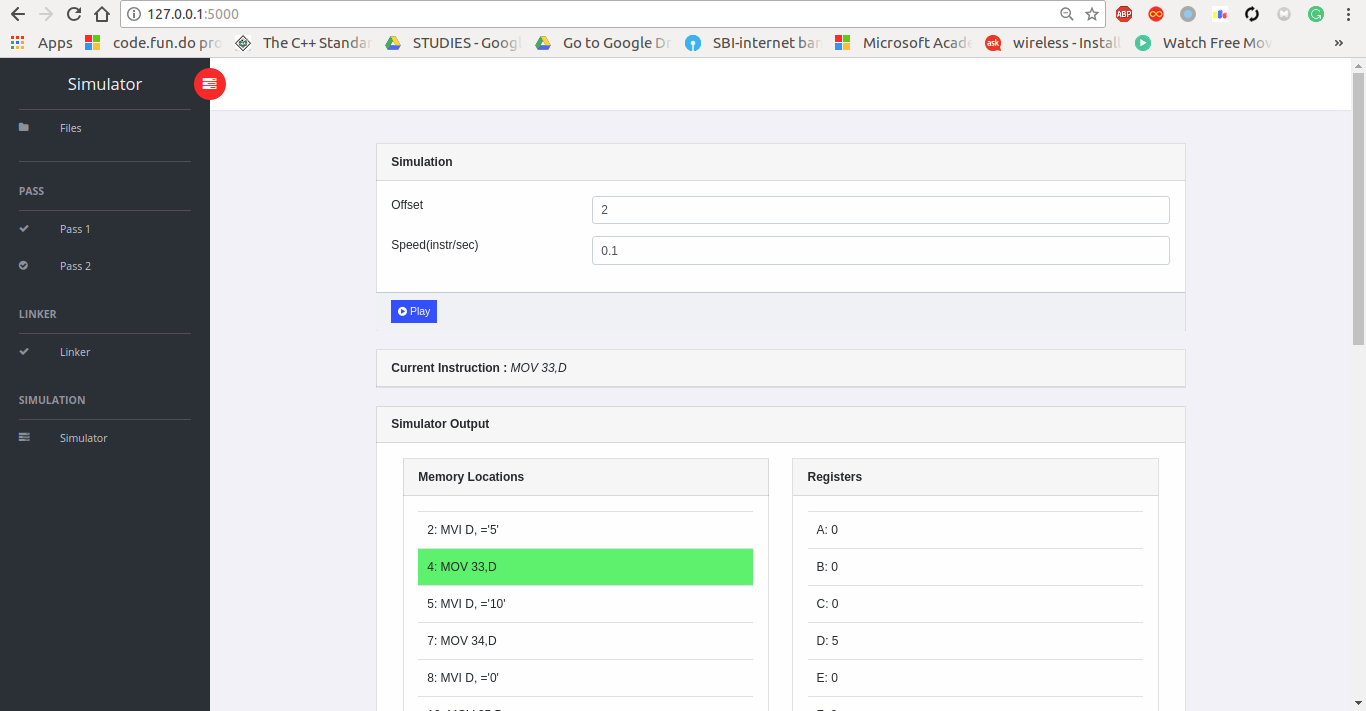
\includegraphics[width=\textwidth, keepaspectratio]{simulator.png}
\caption{Linker window}
\end{figure}

\begin{itemize}
\item[•] To simulate first enter value for offset and speed of execution.
\item[•] Next click on play button.
\item[•] You will see the code will start executing with line under execution highlighted with green.
\end{itemize}

\chapter{Assembler}
\section{Data Structures Used}
\begin{enumerate}

\item \textbf{Location Counter(LC)}
\begin{itemize}
\item[•]To implement memory allocation a data structure called location counter(LC) is introduced.
\item[•]The location counter is always made to contain the address of the mnext memory word in the target program.
\item[•]It is initialised to the constant specified in the START statment.
\item[•]Whenever the analysis phase sees a label and the contents of LC in a new entry of the symbol table.
\item[•]It then finds the number of memeory words required by the assembly statement and updates the LC contents.
\end{itemize}

\item \textbf{Operands Table - OPTAB:}
\begin{itemize}
\item[•]OPTAB contains the fields mnemonic opcode, class and mnemonic info.
\item[•]The class field indicates whether the opcode corresponds  to an imperative statemnts(IS), declaraive statements(DS) or an assembler directive.
\item[•]Next it contains length of mnemonic info - its length and hexcode.
\end{itemize}

\item \textbf{Symbols Table - SYMTAB:}
\begin{itemize}
\item[•]A symbol table contains symbol, adress and length of various variables.
\item[•]While processing of an assembly language it contains label, it is entered into symbol field of symtab and value of location counter is copied into length field.
\item[•]The length of symbol is also entered into symtab if defined in statement.
\item[•]For eg: consider the statement
\begin{center}
a DS 4\\
Symbol: a\\
Length: 4\\
Adress: It will be value of location counter(LC)\\
\end{center}
\end{itemize}

\item \textbf{LITTAB and POOLTAB}
\begin{itemize}
\item[•]The first pass uses LITTAB to collect all literals used in program.
\item[•]Awareness of different literals pools is maintained using the auxillary table POOLTAB.
\item[•]POOLTAB contains the literal number of the starting itera of each literal pool.
\item[•]On encountoring LTORG or END statement all the literals are allocated adresses
\end{itemize}
\end{enumerate}

\section{Pass1 of Assembler}
\subsection{Psuedocode for algorithm used}
\begin{enumerate}
\item LC=0;(default values)
\item[]pooltab_ptr=1; 
\item[]POOLTAB[1]=1;
\item[]littab_ptr=1;
\item While next statement is not an END statement
\begin{enumerate}
\item If label is pesent then 
\begin{itemize}
\item[] this_label= symbol in the label field;
\item[] Enter(this_label, LC) in SYMTAB;
\end{itemize}

\item If START or ORIGIN statement then
\begin{itemize}
\item[] LC = value specified in operand field;
\end{itemize}

\item If an EQU statement then
\begin{enumerate}
\item this_addr = value of $<$adress_spec$>$;
\item Correct the symtab entry for this_label to(this_label, this_addr)
\end{enumerate}

\item If a declaration satement then
\begin{enumerate}
\item code = code of the declaration statement;
\item size = size of memeory area required by DC/DS
\item LC = LC + size;
\item Generate(DL, code)...
\end{enumerate}

\item If an imperative statement then
\begin{enumerate}
\item code  = machine opcode from OPTAB
\item LC = LC + instruction length from OPTAB
\item If operand is a literal then
\begin{itemize}
\item[]this_literal = litera inoperand field;
\item[]LITTAB[littab_ptr]=this_literal;
\item[]littab_ptr = littab_ptr + 1;
\end{itemize}
\item else(i.e. operand is a symbol)
\begin{itemize}
\item[]this_entry = SYMTAB entry number of operand;
\item[]Generate IC
\end{itemize}
\end{enumerate}
\end{enumerate}

\item (Processing of END statement)
\begin{enumerate}
\item Process all literals to allocate memory and put the address field. Update LC accordingly.
\item Generate IC'(AD, 02)'
\item Go to Pass2
\end{enumerate}
\end{enumerate}

\section{Pass1 of Assembler}
\subsection{Psuedocode for algorithm used}
Algorithm 4.2 (Assembler Second Pass)
\begin{enumerate}
\item code_area_address = address of code_area;
\item[] pooltab_ptr z= I;
\item[] loc_cntr = 0;

\item While next statement is not an END statement
\begin{enumerate}
\item Clear machine_code_buffer;

\item If an LTORG statement
\begin{enumerate}
\item Process literals in LIITTAB[POOLTAB[pooltab_ptr]]...LITTAB
   [POOLTAB [pooltab_ptr+1]]-1 similar to processing of constants
in a DC statement, i.e. assemble the literals in machine_code_buffer.
\item size := size of memory area required for literals;
\item pooltab_ptr := pooltab_ptr + 1;
\end{enumerate}

\item If a START or ORIGIN statement then
\begin{enumerate}
\item  loc_cntr := value specified in operand field;
\item size := 0;
\end{enumerate}

\item If a declaration statement
\begin{enumerate}
\item  If a DC statement then
Assemble the constant in machine_code_buffer.
\item size := size of memory area required by DC/DS;
\end{enumerate}

\item If an imperative statement
\begin{enumerate}
\item  Get operand address from SYMTAB or LITT AB.
\item Assemble instruction in machine_code_buffer.
\item size := size of instruction;
\end{enumerate}

\item If size $\neq$ 0 then
\begin{enumerate}
\item  Move contents of machine_code_buffer to the address code_area_address + loc_cntr;
\item loc_cntr := loc_cntr + size;
\end{enumerate}
\end{enumerate}
\item (Processing of END statement)
\begin{enumerate}
\item Perform steps 2(b) and 2(f).
\item Write code_area into output file.
\end{enumerate}

\end{enumerate}

\chapter{Opcode Table of Intel 8085 Processor}
\begin{longtable}{|c|c|c|c|c|c|}
\caption{Opcode Table}\\
\hline
\textbf{First entry} & \textbf{Mnemonic} & \textbf{Fields Entry} & \textbf{Opcode } & \textbf{Length } & \textbf{Length }\\
\hline
\endfirsthead
\multicolumn{5}{c}%
{\tablename\ \thetable\ -- \textit{Continued from previous page}} \\
\hline
\textbf{Ser. No.} & \textbf{Mnemonic} & \textbf{Fields Entry} & \textbf{Opcode } \\
\hline
\endhead
\hline \multicolumn{4}{r}{\textit{Continued on next page}} \\
\endfoot
\hline
\endlastfoot
1.   & ACI  & Data         & CE   & 2  &   \\
2.   & ADC  & A            & 8F   & 1  &   \\
3.   & ADC  & B            & 88   & 1  &   \\
4.   & ADC  & C            & 89   & 1  &   \\
5.   & ADC  & D            & 8A   & 1  &   \\
6.   & ADC  & E            & 8B   & 1  &   \\
7.   & ADC  & H            & 8C   & 1  &   \\
8.   & ADC  & L            & 8D   & 1  &   \\
9.   & ADC  & M            & 8E   & 1  &   \\
10.  & ADD  & A            & 87   & 1  &   \\
11.  & ADD  & B            & 80   & 1  &   \\
12.  & ADD  & C            & 81   & 1  &   \\
13.  & ADD  & D            & 82   & 1  &   \\
14.  & ADD  & E            & 83   & 1  &   \\
15.  & ADD  & H            & 84   & 1  &   \\
16.  & ADD  & L            & 85   & 1  &   \\
17.  & ADD  & M            & 86   & 1  &   \\
18.  & ADI  & Data         & C6   & 2  &   \\
19.  & ANA  & A            & A7   & 1  &   \\
20.  & ANA  & B            & A0   & 1  &   \\
21.  & ANA  & C            & A1   & 1  &   \\
22.  & ANA  & D            & A2   & 1  &   \\
23.  & ANA  & E            & A3   & 1  &   \\
24.  & ANA  & H            & A4   & 1  &   \\
25.  & ANA  & L            & A5   & 1  &   \\
26.  & ANA  & M            & A6   & 1  &   \\
27.  & ANI  & Data         & E6   & 2  &   \\
28.  & CALL & Label        & CD   & 3  &   \\
29.  & CC   & Label        & DC   & 3  &   \\
30.  & CM   & Label        & FC   & 3  &   \\
31.  & CMA  & 2F           & 1    &    &   \\
32.  & CMC  & 3F           & 1    &    &   \\
33.  & CMP  & A            & BF   & 1  &   \\
34.  & CMP  & B            & B8   & 1  &   \\
35.  & CMP  & C            & B9   & 1  &   \\
36.  & CMP  & D            & BA   & 1  &   \\
37.  & CMP  & E            & BB   & 1  &   \\
38.  & CMP  & H            & BC   & 1  &   \\
39.  & CMP  & L            & BD   & 1  &   \\
40.  & CMP  & M            & BD   & 1  &   \\
41.  & CNC  & Label        & D4   & 3  &   \\
42.  & CNZ  & Label        & C4   & 3  &   \\
43.  & CP   & Label        & F4   & 3  &   \\
44.  & CPE  & Label        & EC   & 3  &   \\
45.  & CPI  & Data         & FE   & 2  &   \\
46.  & CPO  & Label        & E4   & 3  &   \\
47.  & CZ   & Label        & CC   & 3  &   \\
48.  & DAA  & 27           & 1    &    &   \\
49.  & DAD  & B            & 09   & 1  &   \\
50.  & DAD  & D            & 19   & 1  &   \\
51.  & DAD  & H            & 29   & 1  &   \\
52.  & DAD  & SP           & 39   & 1  &   \\
53.  & DCR  & A            & 3D   & 1  &   \\
54.  & DCR  & B            & 05   & 1  &   \\
55.  & DCR  & C            & 0D   & 1  &   \\
56.  & DCR  & D            & 15   & 1  &   \\
57.  & DCR  & E            & 1D   & 1  &   \\
58.  & DCR  & H            & 25   & 1  &   \\
59.  & DCR  & L            & 2D   & 1  &   \\
60.  & DCR  & M            & 35   & 1  &   \\
61.  & DCX  & B            & 0B   & 1  &   \\
62.  & DCX  & D            & 1B   & 1  &   \\
63.  & DCX  & H            & 2B   & 1  &   \\
64.  & DCX  & SP           & 3B   & 1  &   \\
65.  & DI   & F3           & 1    &    &   \\
66.  & EI   & FB           & 1    &    &   \\
67.  & HLT  & 76           & 1    &    &   \\
68.  & IN   & Port-address & DB   & 2  &   \\
69.  & INR  & A            & 3C   & 1  &   \\
70.  & INR  & B            & 04   & 1  &   \\
71.  & INR  & C            & 0C   & 1  &   \\
72.  & INR  & D            & 14   & 1  &   \\
73.  & INR  & E            & 1C   & 1  &   \\
74.  & INR  & H            & 24   & 1  &   \\
75.  & INR  & L            & 2C   & 1  &   \\
76.  & INR  & M            & 34   & 1  &   \\
77.  & INX  & B            & 03   & 1  &   \\
78.  & INX  & D            & 13   & 1  &   \\
79.  & INX  & H            & 23   & 1  &   \\
80.  & INX  & SP           & 33   & 1  &   \\
81.  & JC   & Label        & DA   & 3  &   \\
82.  & JM   & Label        & FA   & 3  &   \\
83.  & JMP  & Label        & C3   & 3  &   \\
84.  & JNC  & Label        & D2   & 3  &   \\
85.  & JNZ  & Label        & C2   & 3  &   \\
86.  & JP   & Label        & F2   & 3  &   \\
87.  & JPE  & Label        & EA   & 3  &   \\
88.  & JPO  & Label        & E2   & 3  &   \\
89.  & JZ   & Label        & CA   & 3  &   \\
90.  & LDA  & Address      & 3A   & 3  &   \\
91.  & LDAX & B            & 0A   & 1  &   \\
92.  & LDAX & D            & 1A   & 1  &   \\
93.  & LHLD & Address      & 2A   & 3  &   \\
94.  & LXI  & B            & 01   & 3  &   \\
95.  & LXI  & D            & 11   & 3  &   \\
96.  & LXI  & H            & 21   & 3  &   \\
97.  & LXI  & SP           & 31   & 3  &   \\
98.  & MOV  & A,           & A    & 7F & 1 \\
99.  & MOV  & A,           & B    & 78 & 1 \\
100. & MOV  & A,           & C    & 79 & 1 \\
101. & MOV  & A,           & D    & 7A & 1 \\
102. & MOV  & A,           & E    & 7B & 1 \\
103. & MOV  & A,           & H    & 7C & 1 \\
104. & MOV  & A,           & L    & 7D & 1 \\
105. & MOV  & A,           & M    & 7E & 1 \\
106. & MOV  & B,           & A    & 47 & 1 \\
107. & MOV  & B,           & B    & 40 & 1 \\
108. & MOV  & B,           & C    & 41 & 1 \\
109. & MOV  & B,           & D    & 42 & 1 \\
110. & MOV  & B,           & E    & 43 & 1 \\
111. & MOV  & B,           & H    & 44 & 1 \\
112. & MOV  & B,           & L    & 45 & 1 \\
113. & MOV  & B,           & M    & 46 & 1 \\
114. & MOV  & C,           & A    & 4F & 1 \\
115. & MOV  & C,           & B    & 48 & 1 \\
116. & MOV  & C,           & C    & 49 & 1 \\
117. & MOV  & C,           & D    & 4A & 1 \\
118. & MOV  & C,           & E    & 4B & 1 \\
119. & MOV  & C,           & H    & 4C & 1 \\
120. & MOV  & C,           & L    & 4D & 1 \\
121. & MOV  & C,           & M    & 4E & 1 \\
122. & MOV  & D,           & A    & 57 & 1 \\
123. & MOV  & D,           & B    & 50 & 1 \\
124. & MOV  & D,           & C    & 51 & 1 \\
125. & MOV  & D,           & D    & 52 & 1 \\
126. & MOV  & D,           & E    & 53 & 1 \\
127. & MOV  & D,           & H    & 54 & 1 \\
128. & MOV  & D,           & L    & 55 & 1 \\
129. & MOV  & D,           & M    & 56 & 1 \\
130. & MOV  & E,           & A    & 5F & 1 \\
131. & MOV  & E,           & B    & 58 & 1 \\
132. & MOV  & E,           & C    & 59 & 1 \\
133. & MOV  & E,           & D    & 5A & 1 \\
134. & MOV  & E,           & E    & 5B & 1 \\
135. & MOV  & E,           & H    & 5C & 1 \\
136. & MOV  & E,           & L    & 5D & 1 \\
137. & MOV  & E,           & M    & 5E & 1 \\
138. & MOV  & H,           & A    & 67 & 1 \\
139. & MOV  & H,           & B    & 60 & 1 \\
140. & MOV  & H,           & C    & 61 & 1 \\
141. & MOV  & H,           & D    & 62 & 1 \\
142. & MOV  & H,           & E    & 63 & 1 \\
143. & MOV  & H,           & H    & 64 & 1 \\
144. & MOV  & H,           & L    & 65 & 1 \\
145. & MOV  & H,           & M    & 66 & 1 \\
146. & MOV  & L,           & A    & 6F & 1 \\
147. & MOV  & L,           & B    & 68 & 1 \\
148. & MOV  & L,           & C    & 69 & 1 \\
149. & MOV  & L,           & D    & 6A & 1 \\
150. & MOV  & L,           & E    & 6B & 1 \\
151. & MOV  & L,           & H    & 6C & 1 \\
152. & MOV  & L,           & L    & 6D & 1 \\
153. & MOV  & L,           & M    & 6E & 1 \\
154. & MOV  & M,           & A    & 77 & 1 \\
155. & MOV  & M,           & B    & 70 & 1 \\
156. & MOV  & M,           & C    & 71 & 1 \\
157. & MOV  & M,           & D    & 72 & 1 \\
158. & MOV  & M,           & E    & 73 & 1 \\
159. & MOV  & M,           & H    & 74 & 1 \\
160. & MOV  & M,           & L    & 75 & 1 \\
161. & MVI  & A,           & Data & 3E & 2 \\
162. & MVI  & B,           & Data & 06 & 2 \\
163. & MVI  & C,           & Data & 0E & 2 \\
164. & MVI  & D,           & Data & 16 & 2 \\
165. & MVI  & E,           & Data & 1E & 2 \\
166. & MVI  & H,           & Data & 26 & 2 \\
167. & MVI  & L,           & Data & 2E & 2 \\
168. & MVI  & M,           & Data & 36 & 2 \\
169. & NOP  & 00           & 1    &    &   \\
170. & ORA  & A            & B7   & 1  &   \\
171. & ORA  & B            & B0   & 1  &   \\
172. & ORA  & C            & B1   & 1  &   \\
173. & ORA  & D            & B2   & 1  &   \\
174. & ORA  & E            & B3   & 1  &   \\
175. & ORA  & H            & B4   & 1  &   \\
176. & ORA  & L            & B5   & 1  &   \\
177. & ORA  & M            & B6   & 1  &   \\
178. & ORI  & Data         & F6   & 2  &   \\
179. & OUT  & Port-Address & D3   & 2  &   \\
180. & PCHL & E9           & 1    &    &   \\
181. & POP  & B            & C1   & 1  &   \\
182. & POP  & D            & D1   & 1  &   \\
183. & POP  & H            & E1   & 1  &   \\
184. & POP  & PSW          & F1   & 1  &   \\
185. & PUSH & B            & C5   & 1  &   \\
186. & PUSH & D            & D5   & 1  &   \\
187. & PUSH & H            & E5   & 1  &   \\
188. & PUSH & PSW          & F5   & 1  &   \\
189. & RAL  & 17           & 1    &    &   \\
190. & RAR  & 1F           & 1    &    &   \\
191. & RC   & D8           & 1    &    &   \\
192. & RET  & C9           & 1    &    &   \\
193. & RIM  & 20           & 1    &    &   \\
194. & RLC  & 07           & 1    &    &   \\
195. & RM   & F8           & 1    &    &   \\
196. & RNC  & D0           & 1    &    &   \\
197. & RNZ  & C0           & 1    &    &   \\
198. & RP   & F0           & 1    &    &   \\
199. & RPE  & E8           & 1    &    &   \\
200. & RPO  & E0           & 1    &    &   \\
201. & RRC  & 0F           & 1    &    &   \\
202. & RST  & 0            & C7   & 1  &   \\
203. & RST  & 1            & CF   & 1  &   \\
204. & RST  & 2            & D7   & 1  &   \\
205. & RST  & 3            & DF   & 1  &   \\
206. & RST  & 4            & E7   & 1  &   \\
207. & RST  & 5            & EF   & 1  &   \\
208. & RST  & 6            & F7   & 1  &   \\
209. & RST  & 7            & FF   & 1  &   \\
210. & RZ   & C8           & 1    &    &   \\
211. & SBB  & A            & 9F   & 1  &   \\
212. & SBB  & B            & 98   & 1  &   \\
213. & SBB  & C            & 99   & 1  &   \\
214. & SBB  & D            & 9A   & 1  &   \\
215. & SBB  & E            & 9B   & 1  &   \\
216. & SBB  & H            & 9C   & 1  &   \\
217. & SBB  & L            & 9D   & 1  &   \\
218. & SBB  & M            & 9E   & 1  &   \\
219. & SBI  & Data         & DE   & 2  &   \\
220. & SHLD & Address      & 22   & 3  &   \\
221. & SIM  & 30           & 1    &    &   \\
222. & SPHL & F9           & 1    &    &   \\
223. & STA  & Address      & 32   & 3  &   \\
224. & STAX & B            & 02   & 1  &   \\
225. & STAX & D            & 12   & 1  &   \\
226. & STC  & 37           & 1    &    &   \\
227. & SUB  & A            & 97   & 1  &   \\
228. & SUB  & B            & 90   & 1  &   \\
229. & SUB  & C            & 91   & 1  &   \\
230. & SUB  & D            & 92   & 1  &   \\
231. & SUB  & E            & 93   & 1  &   \\
232. & SUB  & H            & 94   & 1  &   \\
233. & SUB  & L            & 95   & 1  &   \\
234. & SUB  & M            & 96   & 1  &   \\
235. & SUI  & Data         & D6   & 2  &   \\
236. & XCHG & EB           & 1    &    &   \\
237. & XRA  & A            & AF   & 1  &   \\
238. & XRA  & B            & A8   & 1  &   \\
239. & XRA  & C            & A9   & 1  &   \\
240. & XRA  & D            & AA   & 1  &   \\
241. & XRA  & E            & AB   & 1  &   \\
242. & XRA  & H            & AC   & 1  &   \\
243. & XRA  & L            & AD   & 1  &   \\
244. & XRA  & M            & AE   & 1  &   \\
245. & XRI  & Data         & EE   & 2  &   \\
246. & XTHL & E3           & 1    &    &  
\end{longtable}

\chapter{Linker}
\section{Introduction}
It is a tool that mergees the object file produced by seperate compilation or asembly and creates an executable file.
It does its task in three steps;
\begin{enumerate}
\item Searches the progren to find library routines used by
program, e.g. print(), sqrt() and various others.

\item Determines the memory locations that code from each
module wil occupy and relocales its instructions by
adjsting absolute references

\textbf{Relocation:} which modifies the object programs so that it can be loaded at an address different from the location orginally specified.

\item It combines two or more separate cores and supplies the
information needed to allow references between them.

\item Computer programs typically comprise several parts or
modules; all these parts/modules need not be contained within
a single object file, and in such case refer to each other by
means of symbols. Typically, an object file can contain three
kinds of symbols:
\begin{itemize}
\item Publicly defined symbols, which allow it to be called by other
modules , also called as public definition .
\item Externally defined symbols(undefined symbols), which calls
the other modules where these symbols are defined, also
called as external reference.
\item Local symbols, used internally within the object file to facilitate
relocation.  
\end{itemize}
\end{enumerate}


\chapter{Loader}
\section{Introduction}
It is a SYSTEM PROGRAM that brings an executable file
residing on disk into memory and starts it running.
Steps:-
\begin{enumerate}
\item Read executable file’s header to determine the size of
text and data segments.
\item Create a new address space for the program.
\item Copies instructions and data into address space.
\item Copies arguments passed to the program on the stack.
\item Initializes the machine registers including the stack pointer.
\item Jumps to a startup routine that copies the program’s
arguments from the stack to registers and calls the
program’s main routine.
\end{enumerate}

There are mainly four types of loader. We have used a Direct Linking Loader.
Description and their advantages and disadvantages are also mentioned.
\section{Assemble-and-go Loader}

\begin{enumerate}
\item Compilation, assembly, and link steps are not separated
from program execution all in single pass.
\item The intermediate forms of the program are generally kept
in RAM, and not saved to the file system.
\item Compile and go systems differ from interpreters, which
either directly execute source code or execute an
intermediate representation.
\end{enumerate}

\subsection{Advantages}
\begin{enumerate}
\item The user need not be concerned with the separate steps
of compilation, assembling, linking, loading, and
executing.
\item Execution speed is generally much superior to interpreted
systems.
\ They are simple and easier to implement.
\end{enumerate}

\subsection{Disadvantages}
\begin{enumerate}
\item There is wastage in memory space due to the presence of
the assembler.
\item The code must be reprocessed every time it is run.
\item Systems with multiple modules, possibly in different
languages, cannot be handled naturally within this
framework.
\item Compile-and-go systems were popular in academic
environments, where student programs were small,
compiled many times, usually executed quickly and, once
debugged, seldom needed to be re-executed.
\end{enumerate}

\section{Absolute Loader}
It runs as absolute program.
\subsection{Advantage:}
\begin{enumerate}
\item Simple and efficient
\item No linking or relocation
\end{enumerate}

\subsection{Disadvantage:}
\begin{enumerate}
\item Difficult to use subroutine libraries.
\item The need of programmer to state the actual address.
\end{enumerate}

\section{Bootstrap Loader}
\begin{enumerate}
\item Special Type of Absolute Loader.
\item  When a computer is first tuned on or restarted bootstrap
loader is executed.
\item This bootstrap loads the first program to be run by
computer that is the OS.
\item It loads the first address 0x80.
\end{enumerate}

\section{Direct Linking Loader}
\begin{enumerate}
\item This type of loader is a relocating loader.
\item  The loader cannot have the direct access to the source
code.
\item To place the object code 2 types of addresses can be
used:-
\begin{itemize}
\item ABSOLUTE : In this the absolute path of object code is
known and the code is directly loaded in memory.
\item RELATIVE :In this the relative path is known and this
relative path is given by assembler.
\end{itemize}


\end{enumerate}


\subsection{Working}
The assembler should give the following information to the
loader:
\begin{enumerate}
\item The length of the object code segment.
\item A list of external symbols (could be used by diff.
segment).
\item List of External symbols(The segment itself is using)
\item Information about address constants
\item Machine code translation of the source program
\end{enumerate}


\chapter{Language}
This chpater enlists various featurs implemented in the language
\section{Assignment and declaration}
\begin{enumerate}
\item Variable Declaration
\item[] \textbf{Syntax:}\\
\begin{center}
var variable_name
\end{center}

\item Array Declaration
\item[] \textbf{Syntax:}\\
\begin{center}
var array_name[size]
\end{center} 

\item Array Assignment
\item[] \textbf{Syntax:}\\
\begin{center}
array_name[index] = value
\end{center}
\end{enumerate}

\section{Arithematic and Logical Operations}
\begin{enumerate}
\item Addition
\item[] \textbf{Syntax:}\\
\begin{center}
variable_name = variable_name/constant + variable_name/constant
\end{center}

\item Subtraction
\item[] \textbf{Syntax:}\\
\begin{center}
variable_name = variable_name/constant - variable_name/constant
\end{center}

\item Division
\item[] \textbf{Syntax:}\\
\begin{center}
variable_name = variable_name/constant / variable_name/constant
\end{center}

\item Multiplication
\item[] \textbf{Syntax:}\\
\begin{center}
variable_name = variable_name/constant * variable_name/constant
\end{center}

\item Minimum
\item[] \textbf{Syntax:}\\
\begin{center}
variable_name = min({list_of_variables(max 3)})
\end{center}

\item Maximum
\item[] \textbf{Syntax:}\\
\begin{center}
variable_name = max({list_of_variables(max 3)})
\end{center}

\item And
\item[] \textbf{Syntax:}\\
\begin{center}
variable_name = variable_name/constant and_symbol variable_name/constant
\end{center}

\item Or
\item[] \textbf{Syntax:}\\
\begin{center}
variable_name = variable_name/constant or_symbol variable_name/constant
\end{center}
\end{enumerate}

\section{Loop}
\begin{enumerate}
\item for loop
\item[] \textbf{Syntax:}\\
\begin{center}
loop counter\\
Code to be executed
endloop\\
\end{center}

\item nested for loop
\item[] \textbf{Syntax:}\\
\begin{center}
loop counter\\
loop counter\\
Code to be executed\\
endloop\\
endloop\\
\end{center}
\end{enumerate}

\section{If statemnt}
\begin{enumerate}
\item If statement
\item[] \textbf{Syntax:}\\
\begin{center}
If condition\\
Code to be executed
endif\\
\end{center}
\end{enumerate}

\section{Global variables}
\begin{enumerate}
\item global: used for declaring global variables
\item[] \textbf{Syntax:}\\
\begin{center}
global variable_name
\end{center}

\item extern: used for using global variables
\item[] \textbf{Syntax:}\\
\begin{center}
extern variable_name
\end{center}
\end{enumerate}

\section{Macros}
\begin{enumerate}
\item Macro Function
\item[] \textbf{Syntax:}\\
\begin{center}
macro\\
function_name\\
functin_body\\
mend\\
\end{center}

\item Macro Variables
\item[] \textbf{Syntax:}\\
\begin{center}
macro\\
macro_variable_name\\
mend\\
\end{center}
\end{enumerate}

\section{Functions}
\begin{enumerate}
\item  Function: used for declaring global variables
\item[] \textbf{Syntax:}\\
\begin{center}
function function_name\\
function_body\\
endfunction\\
\end{center}
\end{enumerate}

\section{Goto Statements}
\begin{enumerate}
\item  label and jump: used for declaring global variables
\item[] \textbf{Syntax:}\\
\begin{center}
jump: label_name\\
code\\
label_name: code_to_be_executed
\end{center}
\end{enumerate}

\end{document}
